\documentclass{beamer}

\mode<presentation> {
\usepackage{tikz}

% The Beamer class comes with a number of default slide themes
% which change the colors and layouts of slides. Below this is a list
% of all the themes, uncomment each in turn to see what they look like.

%\usetheme{default}
%\usetheme{AnnArbor}
%\usetheme{Antibes}
%\usetheme{Bergen}
%\usetheme{Berkeley}
%\usetheme{Berlin}
%\usetheme{Boadilla}
%\usetheme{CambridgeUS}
%\usetheme{Copenhagen}
%\usetheme{Darmstadt}
%\usetheme{Dresden}
%\usetheme{Frankfurt}
%\usetheme{Goettingen}
%\usetheme{Hannover}
%\usetheme{Ilmenau}
%\usetheme{JuanLesPins}
%\usetheme{Luebeck}
\usetheme{Madrid}
%\usetheme{Malmoe}
%\usetheme{Marburg}
%\usetheme{Montpellier}
%\usetheme{PaloAlto}
%\usetheme{Pittsburgh}
%\usetheme{Rochester}
%\usetheme{Singapore}
%\usetheme{Szeged}
%\usetheme{Warsaw}
\usepackage{amsmath}
% As well as themes, the Beamer class has a number of color themes
% for any slide theme. Uncomment each of these in turn to see how it
% changes the colors of your current slide theme.
\usepackage{array}
%\usecolortheme{albatross}
%\usecolortheme{beaver}
%\usecolortheme{beetle}
%\usecolortheme{crane}
%\usecolortheme{dolphin}
%\usecolortheme{dove}
%\usecolortheme{fly}
%\usecolortheme{lily}
%\usecolortheme{orchid}
%\usecolortheme{rose}
%\usecolortheme{seagull}
%\usecolortheme{seahorse}
%\usecolortheme{whale}
%\usecolortheme{wolverine}

%\setbeamertemplate{footline} % To remove the footer line in all slides uncomment this line
%\setbeamertemplate{footline}[page number] % To replace the footer line in all slides with a simple slide count uncomment this line

%\setbeamertemplate{navigation symbols}{} % To remove the navigation symbols from the bottom of all slides uncomment this line
}

\usepackage{graphicx} % Allows including images
\usepackage{booktabs} % Allows the use of \toprule, \midrule and \bottomrule in tables

%----------------------------------------------------------------------------------------
%	TITLE PAGE
%----------------------------------------------------------------------------------------

\title[Project]{Matrix Project} % The short title appears at the bottom of every slide, the full title is only on the title page

\author{Jayasimha Reddy\and  Rahul Devaraj} % Your name
\institute[IITH] % Your institution as it will appear on the bottom of every slide, may be shorthand to save space
{
IITH\\ % Your institution for the title page
\medskip
\textit{ee15btech11024@iith.ac.in \and ce15btech11002@iith.ac.in} % Your email address
}
\date{\today} % Date, can be changed to a custom date

\begin{document}

\begin{frame}
\titlepage % Print the title page as the first slide
\end{frame}

%----------------------------------------------------------------------------------------
%	PRESENTATION SLIDES
%----------------------------------------------------------------------------------------

\begin{frame}
\frametitle{Geometry Question}
\begin{block}{JEE Problems in Linear
Algebra - Q33}

A circle passes through \begin{bmatrix}
-2 \\ 4
\end{bmatrix}
and touches the y-axis at \begin{bmatrix}
0 \\ 2
\end{bmatrix}
Which one of the following equations can
represent a diameter of this circle?
\newline
\newline
\newline
a)\begin{bmatrix}
4 & 5
\end{bmatrix}x = 6
\newline
\newline
b)\begin{bmatrix}
2 & -3
\end{bmatrix}x + 10 = 0
\newline
\newline
c)\begin{bmatrix}
3 & 4
\end{bmatrix}x = 3
\newline
\newline
d)\begin{bmatrix}
5 & 2
\end{bmatrix}x + 4 = 0


\end{block}
\end{frame}

\begin{frame}
\frametitle{Matrix Transformation of Question}
\begin{block}{JEE Problems in Linear
Algebra - Q3}

\newline Let's say point \begin{bmatrix}
-2 \\ 4
\end{bmatrix} is $P_{1}$, \begin{bmatrix}
0 \\ 2
\end{bmatrix} is $P_{2}$ 
and centre C as \begin{bmatrix}
x \\ 2
\end{bmatrix}
\newline
\newline We know that in a circle $\mid\overline{CP_{1}}\mid = \mid\overline{CP_{2}}\mid$,
\newline
\newline $(P_{1}-C)^T(P_{1}-C)=(P_{2}-C)^T(P_{2}-C)$




\end{block}
\end{frame}

%------------------------------------------------

\begin{frame}
\frametitle{Solution}

\newline $C^T(P_{2}-P_{1})=(C^T(P_{2}-P_{1}))^T$   \hspace{50}$[integer]$
\newline
\newline
\newline $C^T(P_{2}-P_{1})=\dfrac{P{2}^TP_{2}-P_{1}^TP_{1}}{2}=\dfrac{\mid{P_{2}}\mid^2-\mid{P_{1}}\mid^2}{2}$
\newline
\newline
\newline [x & 2]\begin{bmatrix}
2 \\ -2
\end{bmatrix} = \dfrac{\mid{P_{2}}\mid^2-\mid{P_{1}}\mid^2}{2}=-8
\newline
\newline
\newline2x-4=-8
\newline
\newline
\implies x=-2


\end{frame}

\begin{frame}
\frametitle{Solution}



\implies Centre C = \begin{bmatrix} -2 \\ 2 \end{bmatrix}
\newline\newline
\newline \implies $Option a)$ \begin{bmatrix}4 & 5
\end{bmatrix}\begin{bmatrix}
-2 \\ 2
\end{bmatrix} = 6 

\newline

\begin{allign}
\[
2 = 6  \hspace{50}(False)
\]
\end{allign}

\newline \implies $Option b)$ \begin{bmatrix}2 & -3
\end{bmatrix}\begin{bmatrix}
-2 \\ 2
\end{bmatrix} + 10 = 0

\newline

\begin{allign}
\[
-10 + 10 = 0 \hspace{50}(True)
\]
\end{allign}

\end{frame}

%------------------------------------------------



%------------------------------------------------

\begin{frame} % Need to use the fragile option when verbatim is used in the slide
\frametitle{Solution}
 


\newline\implies $Option c) \begin{bmatrix}3 & 4
\end{bmatrix}\begin{bmatrix}
-2 \\ 2
\end{bmatrix} + 10 = 0 

\newline

\begin{allign}
\[
2 = 3 \hspace{50}(False)
\]
\end{allign}

\newline\implies $Option d) \begin{bmatrix}5 & 2
\end{bmatrix}\begin{bmatrix}
-2 \\ 2
\end{bmatrix} + 4 = 0 

\newline

\begin{allign}
\[
-6 + 4 = 0 \hspace{50}(False)
\]
\end{allign}

\end{frame}

%------------------------------------------------

\begin{frame}{Diagram}
\centering 
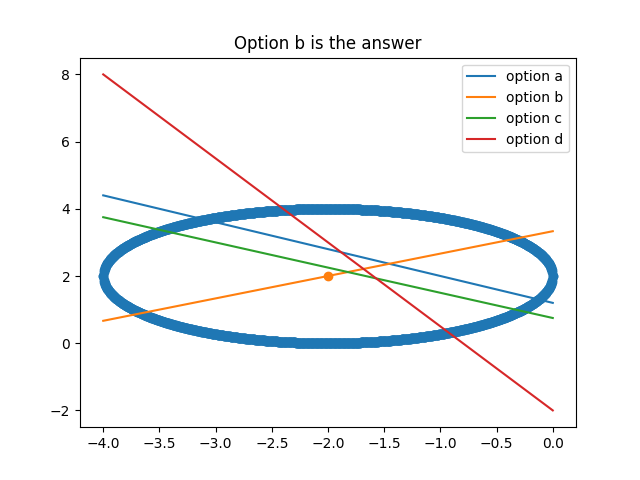
\includegraphics[scale=0.7]{Figure.png}
\end{frame}


%----------------------------------------------------------------------------------------

\end{document}
